\documentclass[11pt]{article}
\usepackage{pifont}
\usepackage{multicol}
\usepackage{listings}
\usepackage{pgf}
\usepackage{tikz}
\usepackage{alltt}
\usepackage{hyperref}
\usepackage{url}
\usepackage{amssymb}
\usetikzlibrary{arrows,automata,shapes,positioning}
\tikzstyle{block} = [rectangle, draw, fill=blue!20, 
    text width=5em, text centered, rounded corners, minimum height=2em]
\tikzstyle{bt} = [rectangle, draw, fill=blue!20, 
    text width=1em, text centered, rounded corners, minimum height=2em]
\newcommand{\xmark}{\ding{55}}

\newtheorem{defn}{Definition}
\newtheorem{crit}{Criterion}
\newcommand{\true}{\mbox{\sf true}}
\newcommand{\false}{\mbox{\sf false}}

\newcommand*\circled[1]{\tikz[baseline=(char.base)]{
            \node[shape=circle,draw,inner sep=2pt] (char) {#1};}}


\newcommand{\handout}[5]{
  \noindent
  \begin{center}
  \framebox{
    \vbox{
      \hbox to 5.78in { {\bf Software Testing, Quality Assurance and Maintenance } \hfill #2 }
      \vspace{4mm}
      \hbox to 5.78in { {\Large \hfill #5  \hfill} }
      \vspace{2mm}
      \hbox to 5.78in { {\em #3 \hfill #4} }
    }
  }
  \end{center}
  \vspace*{4mm}
}

\newcommand{\lecture}[4]{\handout{#1}{#2}{#3}{#4}{Lecture #1}}
\topmargin 0pt
\advance \topmargin by -\headheight
\advance \topmargin by -\headsep
\textheight 8.9in
\oddsidemargin 0pt
\evensidemargin \oddsidemargin
\marginparwidth 0.5in
\textwidth 6.5in

\parindent 0in
\parskip 1.5ex
%\renewcommand{\baselinestretch}{1.25}

\usepackage{enumitem}

\newtheorem{prop}{Proposition}
\newtheorem{lemma}{Lemma}
\usepackage{ebproof}
\newcommand{\qedsymbol}{\rule{1ex}{1ex}}

\lstset{ %
language=Java,
basicstyle=\ttfamily,commentstyle=\scriptsize\itshape,showstringspaces=false,breaklines=true,numbers=left}

%\usepackage{fontspec}
%\setmonofont{Cousine}[Scale=MatchLowercase]

\begin{document}

\lecture{9 --- February 3, 2025}{Winter 2025}{Patrick Lam}{version 1b}

We've talked about symbolic execution, which seems too good to be true, from the examples that we saw.
What? Automatically finding inputs that explore all interesting behaviour? How?

The issue with symbolic executiion is that it's hard to scale. Consider these three problems.
\begin{enumerate}[noitemsep]
\item Code that's hard to analyze: for instance, think of a cryptographic hash function. Smart people have tried to understand how they do what they do. Symbolic execution won't be able to analyze it.
\item Path explosion: the number of paths grows exponentially with the number of nested if statements; handling function calls can also lead to exponential growth; and loops can simply be unbounded.
\item Environment: in the examples we saw, the input was just integers. But in general there might be data structures (and pointers); files and databases; the network, and sockets; and threads (you need to explore all thread schedules).
\end{enumerate}

\paragraph{Example.} Here's a bit of a contrived example.
\begin{lstlisting}
  int obscure(int x, int y) {
    if (x == complex(y))
      error();
    return 0;
  }
\end{lstlisting}
Recall that classical symbolic execution is trying to find inputs that reach all
program points (specifically: cover all paths), including the call to \texttt{error()}.  So, it
considers the \texttt{if} condition \texttt{x == complex(y)}. In the
previous lecture, we had conditions that were just simple arithmetic
and boolean expressions, and hence easy to make either true or false
(by changing the values of the variables in the expressions), using an
SMT solver.  Now, it has to find values for \texttt{x} and \texttt{y}
such that (in this case) \texttt{x == complex(y)}. But
\texttt{complex()} is opaque to the SMT solver, and can be arbitrarily
complicated.

\begin{itemize}[noitemsep]
\item Who is being called? We see \texttt{complex()} here, but that could be
  a virtual function (\texttt{this.complex()}) and we don't necessarily know the
  runtime type of \texttt{this}. Or, it could be a function pointer.
\item Function \texttt{complex()} could be a cryptographic function, like a password hash.
  Now you have to find a password that matches a given hash. Good luck!
\item \texttt{complex()} could contain non-linear integer or floating point arithmetic,
  hard for SMT solvers to reason about.
\item \texttt{complex()} could contain system calls, file I/O, network I/O, etc.
\end{itemize}

\section*{Dynamic Symbolic Execution (DSE)}
We have some tools to mitigate the obstacles to symbolic execution,
under the general name of ``dynamic symbolic execution''.  Symbolic
execution operates completely on symbolic inputs ($X$, $Y$), not
concrete inputs (numbers $17$, $5$).  But sometimes that's hard or
impossible. We thus aim to use concrete execution (as formalized in
the operational semantics) when symbolic execution is hard. The
concrete execution will hopefully guide symbolic execution to useful
parts of the code. This approach is therefore also known as 
\emph{concolic testing} (``\textbf{conc}rete'' +
``symb\textbf{olic}'').

Let's see how it works. Here's the program again.

\begin{lstlisting}
  int obscure(int x, int y) {
    if (x == complex(y))
      error();
    return 0;
  }
\end{lstlisting}
One of the approaches to dynamic symbolic execution is called DART,
for Directed Automated Random Testing. 

\paragraph{Run 1.} So, we'll start with some random inputs.
Let \texttt{x=33} and \texttt{y=42}, which are concrete values you
generated randomly. You concretely run \texttt{complex(42)} and find
that it returns concrete value 567. Since $33 \neq 567$, these inputs lead to the else
branch.

OK, now we want to explore the then-branch. Symbolic execution wants to negate the
\texttt{if}-condition. Oops, that's too hard. Let's instead try running again.
What \texttt{x} should we use? Why not \texttt{x=567}?

\paragraph{Run 2.} This time we are trying with \texttt{x=567} and \texttt{y=42},
as indicated by the previous run. It turns out that \texttt{complex(42)} still returns
567 (it didn't have to, but it does). So the execution goes to the then branch,
covering all branches, and finding the error.

\subsection*{Flavours of Symbolic Execution}
In the previous lecture, we talked about \emph{static symbolic execution} (or classical symbolic execution).
\begin{itemize}[noitemsep]
\item simulates execution on program source code (with symbolic values)
\item starts from entry point, computes strongest post-conditions (symbolically) for the method (by computing them for every program point).
\end{itemize}
Now, we're talking about \emph{dynamic symbolic execution}.
\begin{itemize}[noitemsep]
    \item run/interpret program with concrete state (concrete values)
    \item in parallel, also compute symbolic state alongside concrete state (``concolic'')
    \item occasionally, SMT solver generates new concrete inputs, increasing coverage.
\end{itemize}
Note that the notion of path coverage is key here. We're aiming to increase it.

There are two main flavours of DSE:
\begin{itemize}[noitemsep]
\item EXE-style~\cite{cadar06:_exe}: tools include KLEE (Imperial College London), SPF (NASA), Cloud9, S2E (EPFL)
  \item DART-style~\cite{godefroid05:_dart}: tools include SAGE, PEX (Microsoft), CUTE (UIUC), CREST (UC Berkeley)
\end{itemize}
More on the differences between these later.

\section{EXE}
Let's start by seeing how the EXE-style dynamic symbolic execution works.

\paragraph{Overview.} First, as with the example run we saw before, EXE runs the program concretely, with concrete inputs. You might use fuzzing
or just hard-code some initial inputs.

But, at the same time, EXE runs the symbolic execution in parallel. The symbolic execution follows the concrete execution,
keeping track of which values come from inputs (symbolic) or not (concrete). We've talked about computing path conditions
before, and we'll do that here, using symbolic inputs in the path conditions.

Things get interesting at branch points, where our goal is to explore both cases. At every branch:
\begin{itemize}[noitemsep]
\item concrete execution will take a branch, say branch1.
\item symbolic execution then forces execution into branch2 as well; it updates the input to do that, updating the path condition, and hence creating a new concrete state that reaches branch2.
\end{itemize}
We now have concrete inputs that reach both branch1 and branch2.

\paragraph{Details.} For dynamic symbolic execution, a program state contains a path condition $\mathit{pc}$, as well as values for all variables.
Variables always have a concrete value (in our formalization, an integer), and may have a symbolic value as well (an expression which may contain
input variables e.g. $X$). To start, the state contains mappings to symbolic state like $\mathtt{x}=X$ for all inputs $X$.

At each execution step, we do the following:
\begin{itemize}[noitemsep]
\item update the concrete state by executing a program instruction concretely;
\item update the symbolic state by executing the same instruction symbolically;
\item if the instruction is a branch:
  \begin{itemize}
    \item fork the execution state into two
    \item true branch: conjoin the branch condition to the previous path condition
    \item false branch: conjoin the negated branch condition to the previous path condition (that's how you get in the else branch)
    \item for the branch that the concrete execution didn't take, ask the SMT solver to compute new initial concrete values from the symbolic state. These new inputs must be consistent with the relevant path condition. Replace concrete values with the newly-computed ones, obtaining them by substituting the new inputs into the symbolic state. (This might be impossible, in which case you give up on that path.)
  \end{itemize}
\end{itemize}
Let's look at an example. We did this example with classical symbolic execution, but let's do EXE-style dynamic symbolic execution on it.
\begin{lstlisting}
  int proc(int x) {
    int r = 0;

    if (x > 8) { // (1)
      r = x - 7
    }

    if (x < 5) { // (2)
      r = x - 2;
    }
  }
\end{lstlisting}

Here's our initial state for dynamic symbolic execution.

\begin{center}
    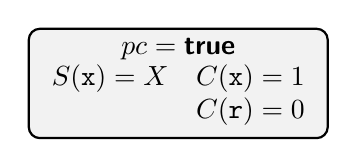
\begin{tikzpicture}[
        node distance=1.5cm and 1cm,
        every node/.style={draw, rounded corners, fill=gray!10, align=center},
        every path/.style={thick},
        decision/.style={draw, rounded corners, fill=gray!20, align=center, minimum width=3.5cm}
    ]


    % Nodes
      \node (start) {\textbf{$pc = \textsf{true}$} \\
        $\begin{array}{ll}
        S(\mathtt{x}) = X & C(\mathtt{x}) = 1 \\
                          & C(\mathtt{r}) = 0
      \end{array}$ };
    
    
    \end{tikzpicture}
\end{center}
The start of the method is always reachable, so \textbf{$pc = \textsf{true}$}. There is one input $X$,
so we have symbolic state $S(\mathtt{x}) = X$. We also have an arbitrarily-drawn concrete value for
\texttt{x}, which is 1, and \texttt{r} will be 0 soon enough.

Let's start executing the program. We have a branch at (1) on condition
$\texttt{x} > 8$. The concrete state $\texttt{x}=1$ drives the concrete execution
into the else branch, indicated by the dotted line.

\begin{center}
    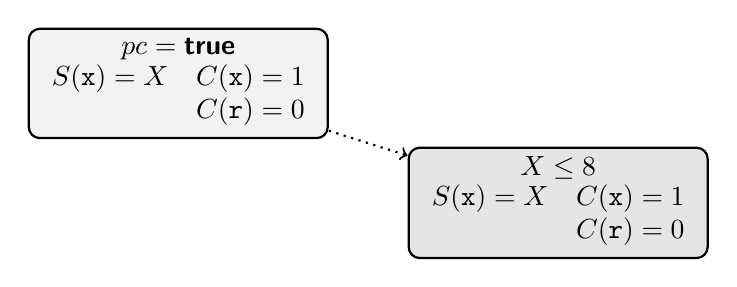
\begin{tikzpicture}[
        node distance=1.5cm and 1cm,
        every node/.style={draw, rounded corners, fill=gray!10, align=center},
        every path/.style={thick},
        decision/.style={draw, rounded corners, fill=gray!20, align=center, minimum width=3.5cm, yshift=2em}
    ]


    % Nodes
      \node (start) {\textbf{$pc = \textsf{true}$} \\
        $\begin{array}{ll}
        S(\mathtt{x}) = X & C(\mathtt{x}) = 1 \\
                          & C(\mathtt{r}) = 0
      \end{array}$ };
    
    \node (right)[below right=of start, decision,yshift=2em] {$X \leq 8$ \\ 
        $\begin{array}{ll}
        S(\mathtt{x}) = X & C(\mathtt{x}) = 1 \\
                          & C(\mathtt{r}) = 0
      \end{array}$ };
    \draw[->, dotted] (start) -- (right);
    
    \end{tikzpicture}
\end{center}
Now we also visit the then-branch. The path condition is simply the branch condition $X > 8$.
We ask the SMT solver to generate a value for $X$ that satisfies $X > 8$; it can ($\checkmark$), and comes back with 9 for $X$
and hence \texttt{x}.
We don't update \texttt{r} since it doesn't depend on $X$.

\begin{center}
    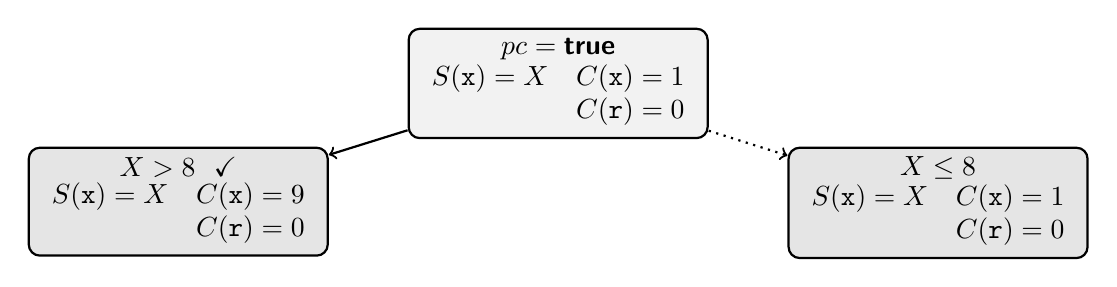
\begin{tikzpicture}[
        node distance=1.5cm and 1cm,
        every node/.style={draw, rounded corners, fill=gray!10, align=center},
        every path/.style={thick},
        decision/.style={draw, rounded corners, fill=gray!20, align=center, minimum width=3.5cm, yshift=2em}
    ]


    % Nodes
      \node (start) {\textbf{$pc = \textsf{true}$} \\
        $\begin{array}{ll}
        S(\mathtt{x}) = X & C(\mathtt{x}) = 1 \\
                          & C(\mathtt{r}) = 0
      \end{array}$ };
    
    \node (left)[below left=of start, decision,yshift=2em] {$X > 8 ~~ \checkmark$ \\ 
        $\begin{array}{ll}
        S(\mathtt{x}) = X & C(\mathtt{x}) = 9 \\
                          & C(\mathtt{r}) = 0
      \end{array}$ };
    \node (right)[below right=of start, decision,yshift=2em] {$X \leq 8$ \\ 
        $\begin{array}{ll}
        S(\mathtt{x}) = X & C(\mathtt{x}) = 1 \\
                          & C(\mathtt{r}) = 0
      \end{array}$ };
    
    % Edges
    \draw[->] (start) -- (left);
    \draw[->, dotted] (start) -- (right);
    
    \end{tikzpicture}
\end{center}
We continue execution on the then-branch, which reassigns \texttt{r}.
\begin{center}
    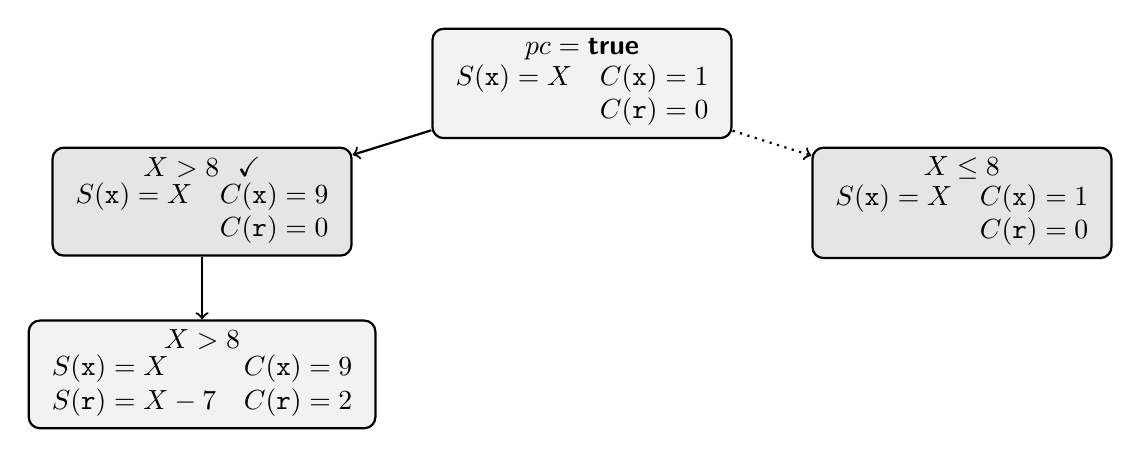
\begin{tikzpicture}[
        node distance=1.5cm and 1cm,
        every node/.style={draw, rounded corners, fill=gray!10, align=center},
        every path/.style={thick},
        decision/.style={draw, rounded corners, fill=gray!20, align=center, minimum width=3.5cm, yshift=2em}
    ]


    % Nodes
      \node (start) {\textbf{$pc = \textsf{true}$} \\
        $\begin{array}{ll}
        S(\mathtt{x}) = X & C(\mathtt{x}) = 1 \\
                          & C(\mathtt{r}) = 0
      \end{array}$ };
    
    \node (left)[below left=of start, decision,yshift=2em] {$X > 8 ~~ \checkmark$ \\ 
        $\begin{array}{ll}
        S(\mathtt{x}) = X & C(\mathtt{x}) = 9 \\
                          & C(\mathtt{r}) = 0
      \end{array}$ };
    \node (left2)[below=of left,yshift=2em] {$X > 8$ \\ 
        $\begin{array}{ll}
        S(\mathtt{x}) = X & C(\mathtt{x}) = 9 \\
        S(\mathtt{r}) = X - 7 & C(\mathtt{r}) = 2
      \end{array}$ };
    \node (right)[below right=of start, decision,yshift=2em] {$X \leq 8$ \\ 
        $\begin{array}{ll}
        S(\mathtt{x}) = X & C(\mathtt{x}) = 1 \\
                          & C(\mathtt{r}) = 0
      \end{array}$ };
    
    % Edges
    \draw[->] (start) -- (left);
    \draw[->] (left) -- (left2);
    \draw[->, dotted] (start) -- (right);
    
    \end{tikzpicture}
\end{center}
Let's continue on this branch with the next if-statement (2). In this case we have concrete \texttt{x} being 9, which runs to the empty else-branch, and thus finishes with no further changes in state.
\begin{center}
    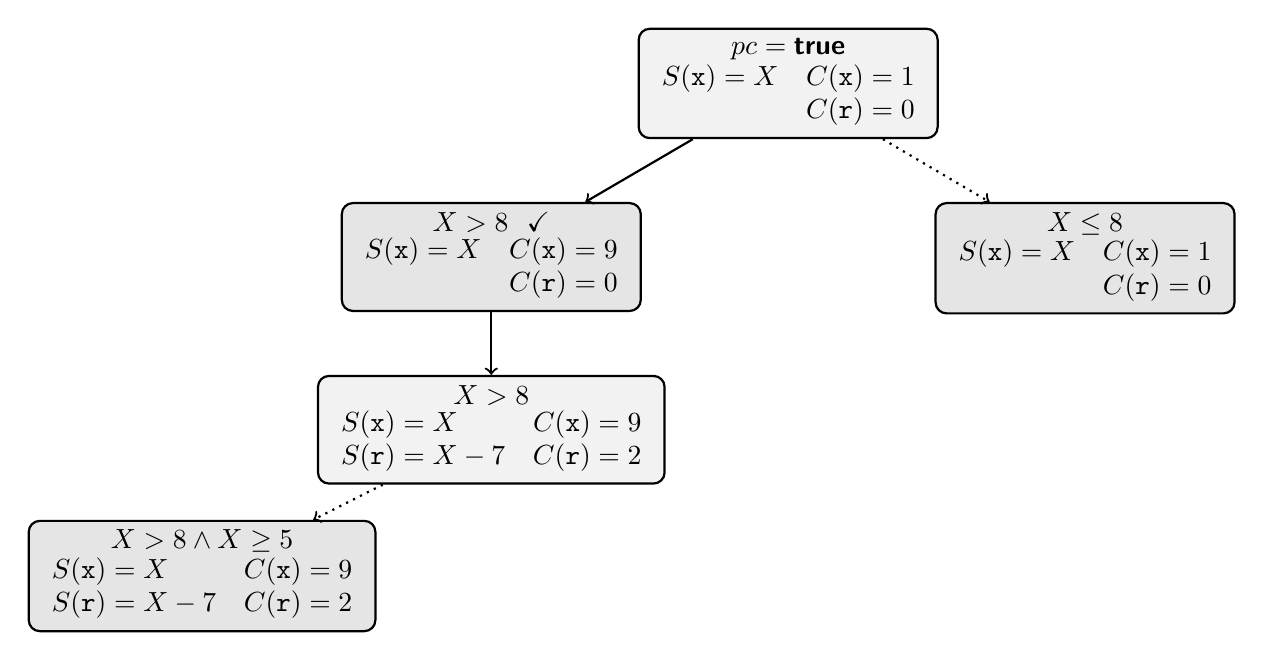
\begin{tikzpicture}[
        node distance=1.5cm and 1cm,
        every node/.style={draw, rounded corners, fill=gray!10, align=center},
        every path/.style={thick},
        decision/.style={draw, rounded corners, fill=gray!20, align=center, minimum width=3.5cm, yshift=2em}
    ]


    % Nodes
      \node (start) {\textbf{$pc = \textsf{true}$} \\
        $\begin{array}{ll}
        S(\mathtt{x}) = X & C(\mathtt{x}) = 1 \\
                          & C(\mathtt{r}) = 0
      \end{array}$ };
    
    \node (left)[below left=of start, decision,xshift=3em] {$X > 8 ~~ \checkmark$ \\ 
        $\begin{array}{ll}
        S(\mathtt{x}) = X & C(\mathtt{x}) = 9 \\
                          & C(\mathtt{r}) = 0
      \end{array}$ };
    \node (left2)[below=of left,yshift=2em] {$X > 8$ \\ 
        $\begin{array}{ll}
        S(\mathtt{x}) = X & C(\mathtt{x}) = 9 \\
        S(\mathtt{r}) = X - 7 & C(\mathtt{r}) = 2
      \end{array}$ };
    \node (left3)[below left=of left2,decision,xshift=5em,yshift=1em] {$X > 8 \wedge X \ge 5$ \\ 
        $\begin{array}{ll}
        S(\mathtt{x}) = X & C(\mathtt{x}) = 9 \\
        S(\mathtt{r}) = X - 7 & C(\mathtt{r}) = 2
      \end{array}$ };
    
    \node (right)[below right=of start, decision,xshift=-3em] {$X \leq 8$ \\ 
        $\begin{array}{ll}
        S(\mathtt{x}) = X & C(\mathtt{x}) = 1 \\
                          & C(\mathtt{r}) = 0
      \end{array}$ };
    
    % Edges
    \draw[->] (start) -- (left);
    \draw[->] (left) -- (left2);
    \draw[->,dotted] (left2) -- (left3);
    \draw[->, dotted] (start) -- (right);
    
    \end{tikzpicture}
\end{center}
The other possibility is the then-branch of (2). Let's try that.
\begin{center}
    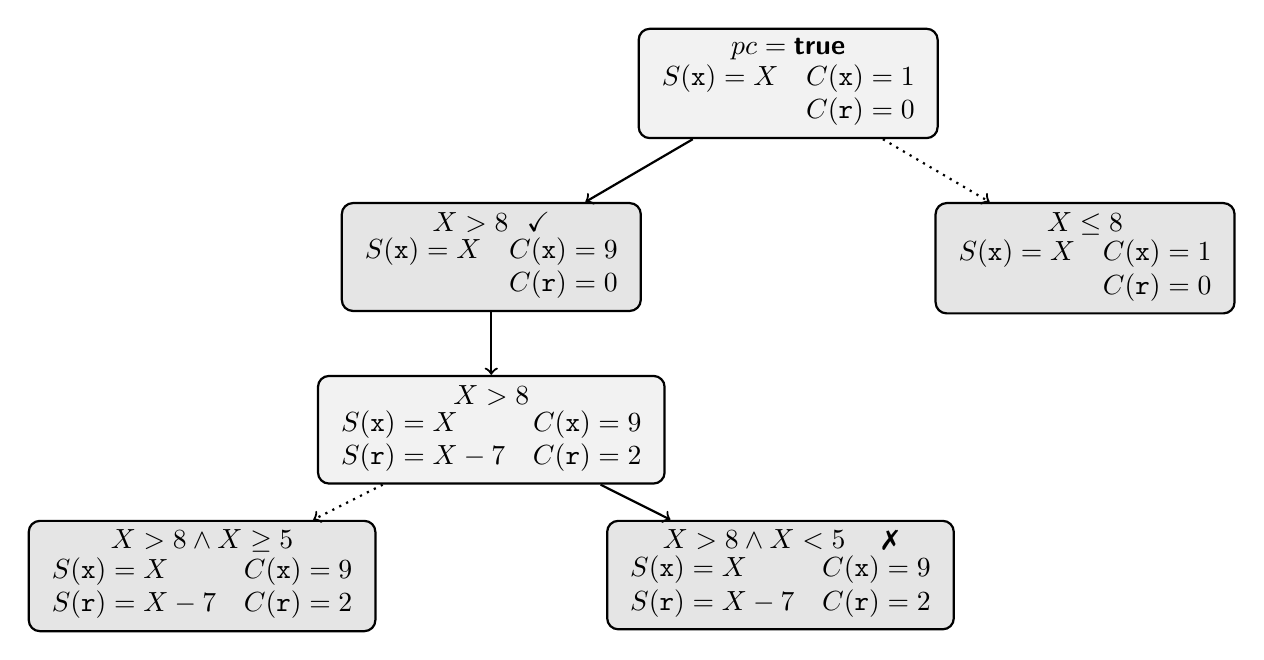
\begin{tikzpicture}[
        node distance=1.5cm and 1cm,
        every node/.style={draw, rounded corners, fill=gray!10, align=center},
        every path/.style={thick},
        decision/.style={draw, rounded corners, fill=gray!20, align=center, minimum width=3.5cm, yshift=2em}
    ]


    % Nodes
      \node (start) {\textbf{$pc = \textsf{true}$} \\
        $\begin{array}{ll}
        S(\mathtt{x}) = X & C(\mathtt{x}) = 1 \\
                          & C(\mathtt{r}) = 0
      \end{array}$ };
    
    \node (left)[below left=of start, decision,xshift=3em] {$X > 8 ~~ \checkmark$ \\ 
        $\begin{array}{ll}
        S(\mathtt{x}) = X & C(\mathtt{x}) = 9 \\
                          & C(\mathtt{r}) = 0
      \end{array}$ };
    \node (left2)[below=of left,yshift=2em] {$X > 8$ \\ 
        $\begin{array}{ll}
        S(\mathtt{x}) = X & C(\mathtt{x}) = 9 \\
        S(\mathtt{r}) = X - 7 & C(\mathtt{r}) = 2
      \end{array}$ };
    \node (left3)[below left=of left2,decision,xshift=5em,yshift=1em] {$X > 8 \wedge X \ge 5$ \\ 
        $\begin{array}{ll}
        S(\mathtt{x}) = X & C(\mathtt{x}) = 9 \\
        S(\mathtt{r}) = X - 7 & C(\mathtt{r}) = 2
      \end{array}$ };
    \node (left3b)[below right=of left2,decision,xshift=-5em,yshift=1em] {$X > 8 \wedge X < 5$ ~~ \xmark \\ 
        $\begin{array}{ll}
        S(\mathtt{x}) = X & C(\mathtt{x}) = 9 \\
        S(\mathtt{r}) = X - 7 & C(\mathtt{r}) = 2
      \end{array}$ };
    
    \node (right)[below right=of start, decision,xshift=-3em] {$X \leq 8$ \\ 
        $\begin{array}{ll}
        S(\mathtt{x}) = X & C(\mathtt{x}) = 1 \\
                          & C(\mathtt{r}) = 0
      \end{array}$ };
    
    % Edges
    \draw[->] (start) -- (left);
    \draw[->] (left) -- (left2);
    \draw[->,dotted] (left2) -- (left3);
    \draw[->] (left2) -- (left3b);
    \draw[->, dotted] (start) -- (right);
    
    \end{tikzpicture}
\end{center}
We have an unsatisfiable (\xmark) path condition $X > 8 \wedge X < 5$ so we give up.

We've now completely explored the then-branch of (1). We still haven't finished
exploring the else-branch of (1), so we continue executing it until we reach (2).
In this case, the concrete state says to execute the then-branch of (2) because
$1 < 5$.
\begin{center}
    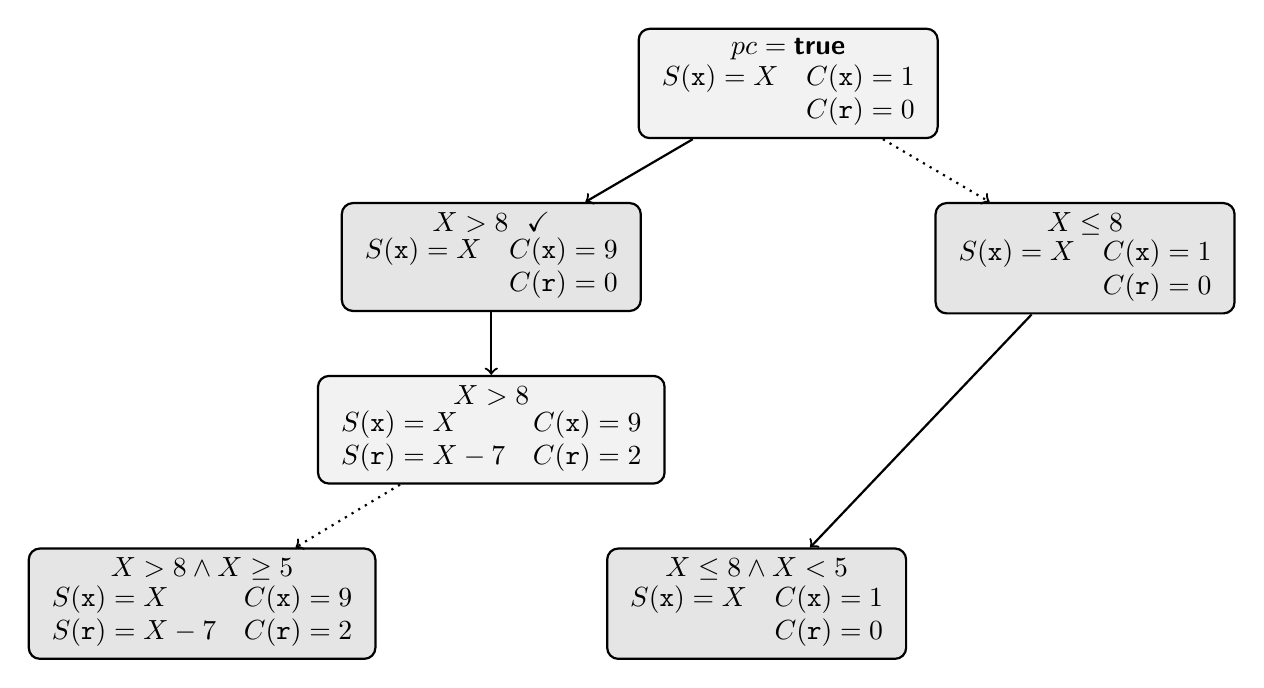
\begin{tikzpicture}[
        node distance=1.5cm and 1cm,
        every node/.style={draw, rounded corners, fill=gray!10, align=center},
        every path/.style={thick},
        decision/.style={draw, rounded corners, fill=gray!20, align=center, minimum width=3.5cm, yshift=2em}
    ]


    % Nodes
      \node (start) {\textbf{$pc = \textsf{true}$} \\
        $\begin{array}{ll}
        S(\mathtt{x}) = X & C(\mathtt{x}) = 1 \\
                          & C(\mathtt{r}) = 0
      \end{array}$ };
    
    \node (left)[below left=of start, decision,xshift=3em] {$X > 8 ~~ \checkmark$ \\ 
        $\begin{array}{ll}
        S(\mathtt{x}) = X & C(\mathtt{x}) = 9 \\
                          & C(\mathtt{r}) = 0
      \end{array}$ };
    \node (left2)[below=of left,yshift=2em] {$X > 8$ \\ 
        $\begin{array}{ll}
        S(\mathtt{x}) = X & C(\mathtt{x}) = 9 \\
        S(\mathtt{r}) = X - 7 & C(\mathtt{r}) = 2
      \end{array}$ };
    \node (left3)[below left=of left2,decision,xshift=5em] {$X > 8 \wedge X \ge 5$ \\ 
        $\begin{array}{ll}
        S(\mathtt{x}) = X & C(\mathtt{x}) = 9 \\
        S(\mathtt{r}) = X - 7 & C(\mathtt{r}) = 2
      \end{array}$ };
    
    \node (right)[below right=of start, decision,xshift=-3em] {$X \leq 8$ \\ 
        $\begin{array}{ll}
        S(\mathtt{x}) = X & C(\mathtt{x}) = 1 \\
                          & C(\mathtt{r}) = 0
      \end{array}$ };
    \node (right2)[below right=of left2,decision,xshift=-5em] {$X \le 8 \wedge X < 5$ \\ 
        $\begin{array}{ll}
        S(\mathtt{x}) = X & C(\mathtt{x}) = 1 \\
                          & C(\mathtt{r}) = 0
      \end{array}$ };
    
    % Edges
    \draw[->] (start) -- (left);
    \draw[->] (left) -- (left2);
    \draw[->,dotted] (left2) -- (left3);
    \draw[->] (right) -- (right2);
    \draw[->, dotted] (start) -- (right);
    
    \end{tikzpicture}
\end{center}
Let's put that on hold for now and explore the else-branch of (2). Here we falsify its branch condition
and successfully $(\checkmark)$ find $X = 6$ as a solution to that path constraint, thus setting $\texttt{x} = 6$.
\begin{center}
    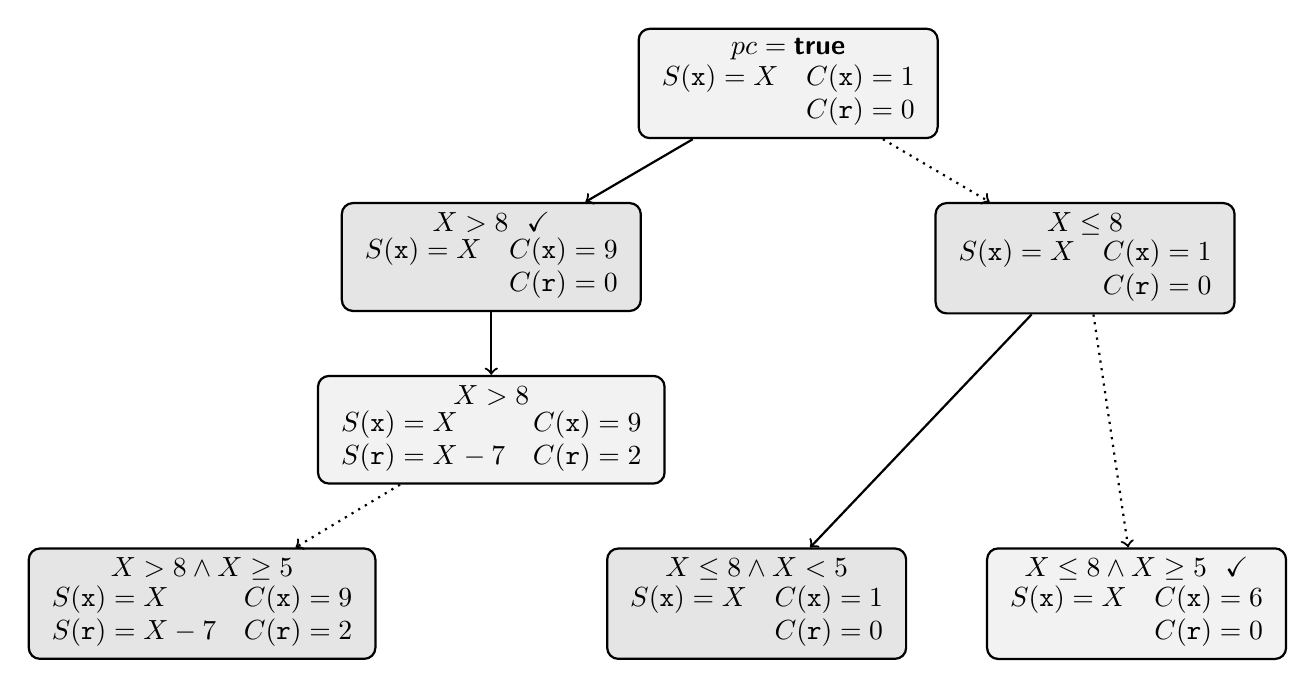
\begin{tikzpicture}[
        node distance=1.5cm and 1cm,
        every node/.style={draw, rounded corners, fill=gray!10, align=center},
        every path/.style={thick},
        decision/.style={draw, rounded corners, fill=gray!20, align=center, minimum width=3.5cm, yshift=2em}
    ]


    % Nodes
      \node (start) {\textbf{$pc = \textsf{true}$} \\
        $\begin{array}{ll}
        S(\mathtt{x}) = X & C(\mathtt{x}) = 1 \\
                          & C(\mathtt{r}) = 0
      \end{array}$ };
    
    \node (left)[below left=of start, decision,xshift=3em] {$X > 8 ~~ \checkmark$ \\ 
        $\begin{array}{ll}
        S(\mathtt{x}) = X & C(\mathtt{x}) = 9 \\
                          & C(\mathtt{r}) = 0
      \end{array}$ };
    \node (left2)[below=of left,yshift=2em] {$X > 8$ \\ 
        $\begin{array}{ll}
        S(\mathtt{x}) = X & C(\mathtt{x}) = 9 \\
        S(\mathtt{r}) = X - 7 & C(\mathtt{r}) = 2
      \end{array}$ };
    \node (left3)[below left=of left2,decision,xshift=5em] {$X > 8 \wedge X \ge 5$ \\ 
        $\begin{array}{ll}
        S(\mathtt{x}) = X & C(\mathtt{x}) = 9 \\
        S(\mathtt{r}) = X - 7 & C(\mathtt{r}) = 2
      \end{array}$ };
    
    \node (right)[below right=of start, decision,xshift=-3em] {$X \leq 8$ \\ 
        $\begin{array}{ll}
        S(\mathtt{x}) = X & C(\mathtt{x}) = 1 \\
                          & C(\mathtt{r}) = 0
      \end{array}$ };
    \node (right2)[below right=of left2,decision,xshift=-5em] {$X \le 8 \wedge X < 5$ \\ 
        $\begin{array}{ll}
        S(\mathtt{x}) = X & C(\mathtt{x}) = 1 \\
                          & C(\mathtt{r}) = 0
      \end{array}$ };
    \node (right2b)[right=of right2] {$X \le 8 \wedge X \ge 5 ~~ \checkmark$ \\ 
        $\begin{array}{ll}
        S(\mathtt{x}) = X & C(\mathtt{x}) = 6 \\
                          & C(\mathtt{r}) = 0
      \end{array}$ };
    
    % Edges
    \draw[->] (start) -- (left);
    \draw[->] (left) -- (left2);
    \draw[->,dotted] (left2) -- (left3);
    \draw[->] (right) -- (right2);
    \draw[->,dotted] (right) -- (right2b);
    \draw[->, dotted] (start) -- (right);
    
    \end{tikzpicture}
\end{center}
Finally, we finish unfinished business with the then-branch of (2) and run through the body of that conditional.
\begin{center}
    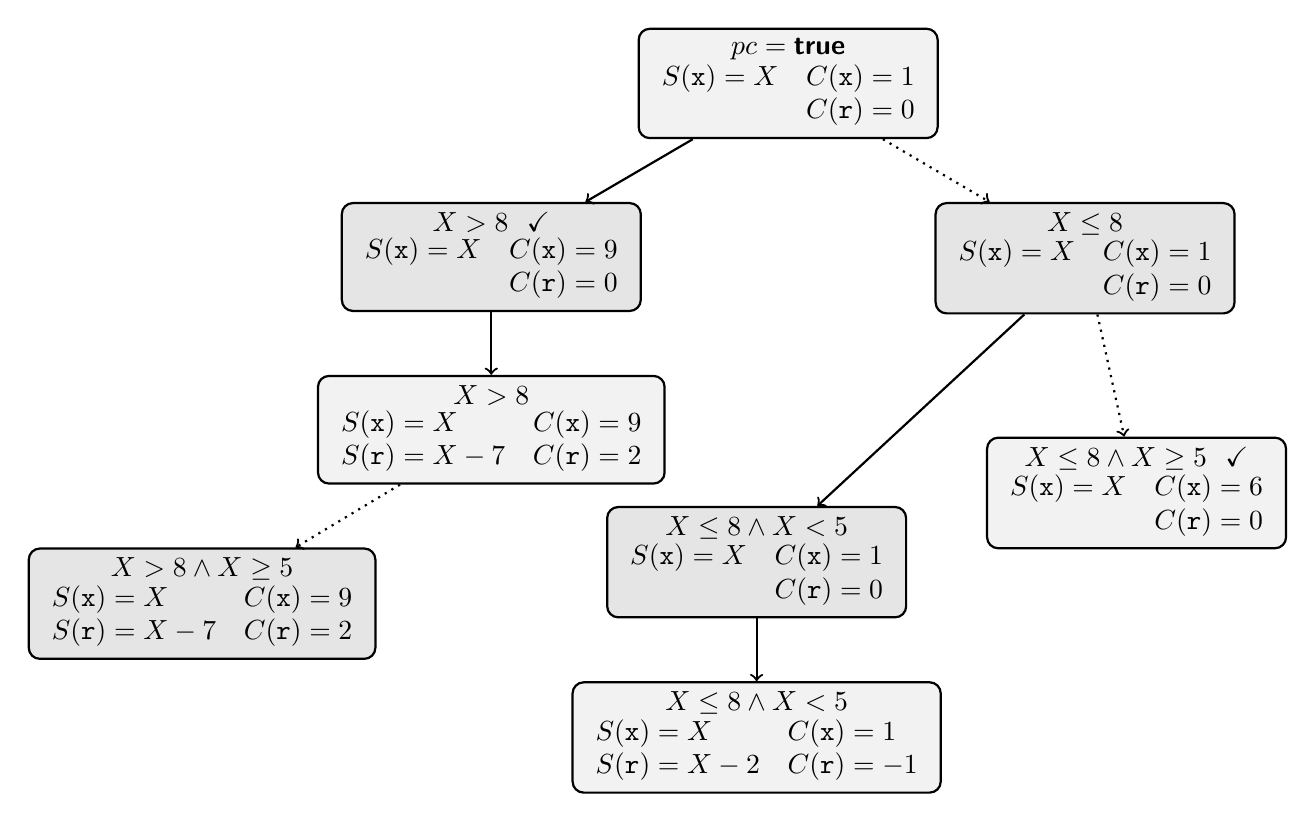
\begin{tikzpicture}[
        node distance=1.5cm and 1cm,
        every node/.style={draw, rounded corners, fill=gray!10, align=center},
        every path/.style={thick},
        decision/.style={draw, rounded corners, fill=gray!20, align=center, minimum width=3.5cm, yshift=2em}
    ]


    % Nodes
      \node (start) {\textbf{$pc = \textsf{true}$} \\
        $\begin{array}{ll}
        S(\mathtt{x}) = X & C(\mathtt{x}) = 1 \\
                          & C(\mathtt{r}) = 0
      \end{array}$ };
    
    \node (left)[below left=of start, decision,xshift=3em] {$X > 8 ~~ \checkmark$ \\ 
        $\begin{array}{ll}
        S(\mathtt{x}) = X & C(\mathtt{x}) = 9 \\
                          & C(\mathtt{r}) = 0
      \end{array}$ };
    \node (left2)[below=of left,yshift=2em] {$X > 8$ \\ 
        $\begin{array}{ll}
        S(\mathtt{x}) = X & C(\mathtt{x}) = 9 \\
        S(\mathtt{r}) = X - 7 & C(\mathtt{r}) = 2
      \end{array}$ };
    \node (left3)[below left=of left2,decision,xshift=5em] {$X > 8 \wedge X \ge 5$ \\ 
        $\begin{array}{ll}
        S(\mathtt{x}) = X & C(\mathtt{x}) = 9 \\
        S(\mathtt{r}) = X - 7 & C(\mathtt{r}) = 2
      \end{array}$ };
    
    \node (right)[below right=of start, decision,xshift=-3em] {$X \leq 8$ \\ 
        $\begin{array}{ll}
        S(\mathtt{x}) = X & C(\mathtt{x}) = 1 \\
                          & C(\mathtt{r}) = 0
      \end{array}$ };
    \node (right2)[below right=of left2,decision,xshift=-5em,yshift=1.5em] {$X \le 8 \wedge X < 5$ \\ 
        $\begin{array}{ll}
        S(\mathtt{x}) = X & C(\mathtt{x}) = 1 \\
                          & C(\mathtt{r}) = 0
      \end{array}$ };
    \node (right21)[below=of right2,yshift=2em] {$X \le 8 \wedge X < 5$ \\ 
        $\begin{array}{ll}
        S(\mathtt{x}) = X & C(\mathtt{x}) = 1 \\
        S(\mathtt{r}) = X-2 & C(\mathtt{r}) = -1
      \end{array}$ };
    \node (right2b)[right=of right2,yshift=2.5em] {$X \le 8 \wedge X \ge 5 ~~ \checkmark$ \\ 
        $\begin{array}{ll}
        S(\mathtt{x}) = X & C(\mathtt{x}) = 6 \\
                          & C(\mathtt{r}) = 0
      \end{array}$ };
    
    % Edges
    \draw[->] (start) -- (left);
    \draw[->] (left) -- (left2);
    \draw[->,dotted] (left2) -- (left3);
    \draw[->] (right) -- (right2);
    \draw[->] (right2) -- (right21);
    \draw[->,dotted] (right) -- (right2b);
    \draw[->, dotted] (start) -- (right);
    
    \end{tikzpicture}
\end{center}
Throughout the dynamic symbolic execution, we collected satisfying assignments $X = 9$, $X = 1$, and $X = 6$, yielding test cases
\texttt{proc(9)}, \texttt{proc(1)}, \texttt{proc(6)}.

\paragraph{EXE: Implementation considerations.} An implementation of EXE needs to maintain multiple execution states while running the program, with both
symbolic and concrete components. As we saw, we need to switch back and forth between different program points and states. The answer is a special-purpose virtual machine.

KLEE (\url{klee.github.io}) uses the LLVM bitcode interpreter to maintain and update state. This means that programs to be run under KLEE need to be compiled into LLVM bitcode.
You can't compile everything into bitcode though, especially assembly, system calls, and some third-party libraries.

S$^2$E (\url{s2e.systems}) instead uses the QEMU virtual machine to fork and restore the entire machine state, including the operating system. It can therefore execute everything.
It executes any code from the executable of interest symbolically. There's still the problem with system code (the code that couldn't be compiled into bitcode), and it runs that
code concretely. Under-the-hood, it uses LLVM.

\section{DART: Directed Automated Random Testing}
Besides EXE, the other approach is DART. Here, we test the (entire) program concretely, recording the execution paths taken in each run, and then use symbolic execution to compute new inputs.

For the concrete runs, we can use random inputs (from fuzzing), user-provided inputs (from tests), or both. We instrument the program to record execution paths (similar to measuring
path coverage), typically at binary level.

Given a run, we can then re-execute the program symbolically and compute path conditions along the way. As with EXE, at each branch condition, we adjust inputs to force
that a different branch run, yielding new inputs that cover new execution paths.

We can repeat the concrete run/adjust input loop until we run out of time, or (ha, ha) we find all bugs.

There is pseudocode in the slides, but I think Wikipedia's description\footnote{\url{https://en.wikipedia.org/wiki/Concolic_testing}} is actually more clear, and I'll excerpt it here. It's not exactly what we do, since we have both symbolic and concrete values for variables sometimes.
\begin{enumerate}[noitemsep]
\item    Classify a particular set of variables as \emph{input variables}. These variables will be treated as symbolic variables during symbolic execution. All other variables will be treated as concrete values.
\item    Instrument the program so that each operation which may affect a symbolic variable value or a path condition is logged to a trace file, as well as any error that occurs.
\item    Choose an arbitrary input to begin with.
\item    Execute the program.
\item    Symbolically re-execute the program on the trace, generating a set of symbolic constraints (including path conditions).
\item    Negate the last path condition not already negated in order to visit a new execution path. If there is no such path condition, the algorithm terminates.
\item    Invoke an automated satisfiability solver [SMT solver] on the new set of path conditions to generate a new input. If there is no input satisfying the constraints, return to step 6 to try the next execution path.
\item    Return to step 4.
\end{enumerate}

%% Here's some pseudocode.
%% \begin{lstlisting}[escapeinside={(*}{*)}]
%%   formula Seen := False
%%   while (*$\neg$*)Seen is satisfiable do
%%     find input (*$x$*) that satisfies (*$\neg$*)Seen
%%     execute (*$P(x)$*) and record path condition (*$C$*)
%%     // important: (*$x$*) satisfies (*$C$*)
%%     Seen := Seen (*$\vee$*) (*$C$*) // record (*$C$*) as seen
%%   done
%% \end{lstlisting}
%% Here:
%% \begin{itemize}[noitemsep]
%% \item \texttt{Seen} is a formula, recording what path conditions we've seen
%% \item $P$ is the program
%% \item $x$ is a program input (one or multiple values; command-line parameters, input files, etc\ldots)
%% \item $C$ is a path condition, computed using symbolic execution, based on the program path induced by input $x$
%% \end{itemize}

Let's run through the same program as from EXE again. I don't need to show the concrete execution step-by-step; DART runs it all through, anyway. We are again starting with input \texttt{x = 1}, i.e.
test case \texttt{proc(1)}.

\begin{tabular}{ll}
\begin{minipage}{.4\textwidth}
\begin{lstlisting}
  int proc(int x) {
    int r = 0;

    if (x > 8) { // (1)
      r = x - 7
    }

    if (x < 5) { // (2)
      r = x - 2;
    }
  }
\end{lstlisting}
\end{minipage}
&
\begin{minipage}{.55\textwidth}
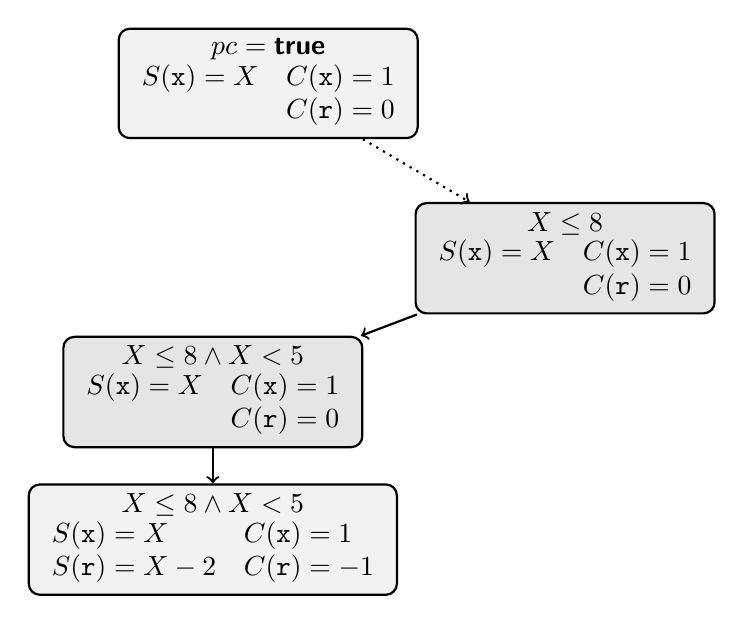
\begin{tikzpicture}[
        node distance=1.5cm and 1cm,
        every node/.style={draw, rounded corners, fill=gray!10, align=center},
        every path/.style={thick},
        decision/.style={draw, rounded corners, fill=gray!20, align=center, minimum width=3.5cm, yshift=2em}
    ]


    % Nodes
      \node (start) {\textbf{$pc = \textsf{true}$} \\
        $\begin{array}{ll}
        S(\mathtt{x}) = X & C(\mathtt{x}) = 1 \\
                          & C(\mathtt{r}) = 0
      \end{array}$ };
    
    \node (right)[below right=of start, decision,xshift=-3em] {$X \leq 8$ \\ 
        $\begin{array}{ll}
        S(\mathtt{x}) = X & C(\mathtt{x}) = 1 \\
                          & C(\mathtt{r}) = 0
      \end{array}$ };
    \node (right2)[below left=of right,decision,xshift=1em,yshift=1.5em] {$X \le 8 \wedge X < 5$ \\ 
        $\begin{array}{ll}
        S(\mathtt{x}) = X & C(\mathtt{x}) = 1 \\
                          & C(\mathtt{r}) = 0
      \end{array}$ };
    \node (right3)[below=of right2,yshift=3em] {$X \le 8 \wedge X < 5$ \\ 
        $\begin{array}{ll}
        S(\mathtt{x}) = X & C(\mathtt{x}) = 1 \\
        S(\mathtt{r}) = X-2 & C(\mathtt{r}) = -1
      \end{array}$ };
    
    % Edges
    \draw[->, dotted] (start) -- (right);
    \draw[->] (right) -- (right2);
    \draw[->] (right2) -- (right3);
    
\end{tikzpicture}
\end{minipage}
\end{tabular}

Looking at the execution, the last path condition occurred at (2) where we had \texttt{x < 5}. We therefore negate it to form the new path condition
$X \le 8 \wedge \neg(X < 5)$; the SMT solver tells us that it is satisfiable ($\checkmark$) and gives us solution $x = 6$, i.e. test case \texttt{proc(6)}.
We run this test case and paste the new state onto the picture.
Really, there are different nodes in the tree for the new run, from the root,
but I don't know how to represent that, so I'm just leaving the old nodes in place.
There are really multiple overlapping nodes; e.g., for the root we also have
a state with $C(\texttt{x}) = 6$.

\begin{center}
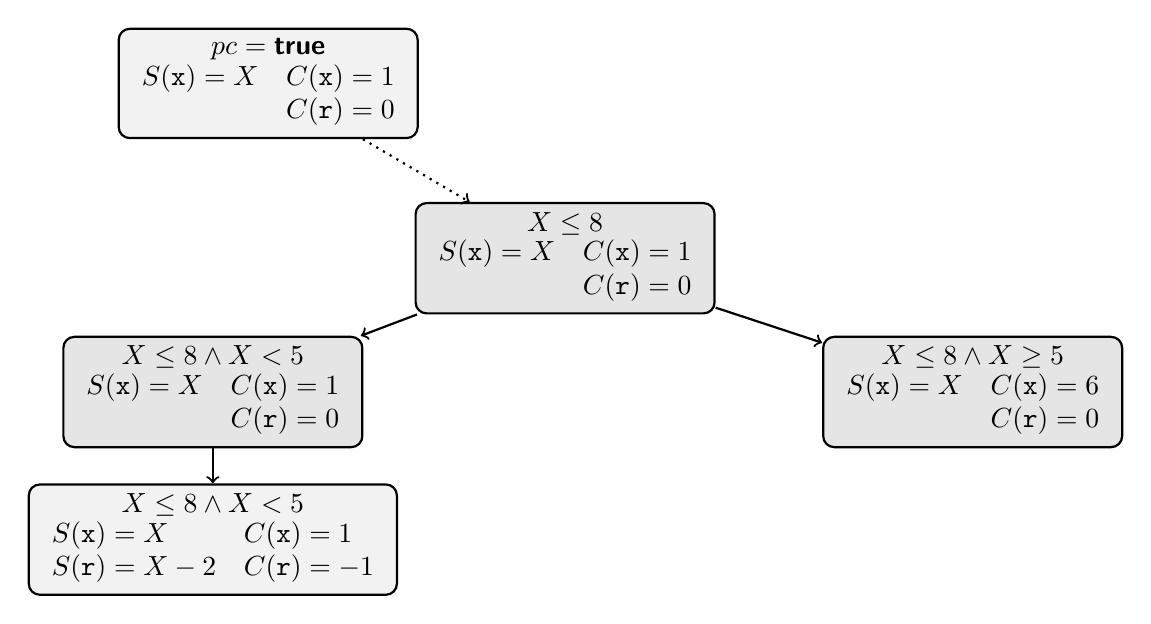
\begin{tikzpicture}[
        node distance=1.5cm and 1cm,
        every node/.style={draw, rounded corners, fill=gray!10, align=center},
        every path/.style={thick},
        decision/.style={draw, rounded corners, fill=gray!20, align=center, minimum width=3.5cm, yshift=2em}
    ]


    % Nodes
      \node (start) {\textbf{$pc = \textsf{true}$} \\
        $\begin{array}{ll}
        S(\mathtt{x}) = X & C(\mathtt{x}) = 1 \\
                          & C(\mathtt{r}) = 0
      \end{array}$ };
    
    \node (right)[below right=of start, decision,xshift=-3em] {$X \leq 8$ \\ 
        $\begin{array}{ll}
        S(\mathtt{x}) = X & C(\mathtt{x}) = 1 \\
                          & C(\mathtt{r}) = 0
      \end{array}$ };
    \node (right2)[below left=of right,decision,xshift=1em,yshift=1.5em] {$X \le 8 \wedge X < 5$ \\ 
        $\begin{array}{ll}
        S(\mathtt{x}) = X & C(\mathtt{x}) = 1 \\
                          & C(\mathtt{r}) = 0
      \end{array}$ };
    \node (right3)[below=of right2,yshift=3em] {$X \le 8 \wedge X < 5$ \\ 
        $\begin{array}{ll}
        S(\mathtt{x}) = X & C(\mathtt{x}) = 1 \\
        S(\mathtt{r}) = X-2 & C(\mathtt{r}) = -1
      \end{array}$ };
    \node (right2b)[below right=of right,decision,xshift=1em,yshift=1.5em] {$X \le 8 \wedge X \ge 5$ \\ 
        $\begin{array}{ll}
        S(\mathtt{x}) = X & C(\mathtt{x}) = 6 \\
                          & C(\mathtt{r}) = 0
      \end{array}$ };
    
    % Edges
    \draw[->, dotted] (start) -- (right);
    \draw[->] (right) -- (right2);
    \draw[->] (right) -- (right2b);
    \draw[->] (right2) -- (right3);
    
\end{tikzpicture}
\end{center}
Because this execution, where \texttt{x=6}, doesn't enter the then-case of (2), this is the end of the execution for \texttt{proc(6)}, and
we've fully explored this part of the space. We back up to (1) and negate that path condition, giving us
new path condition $\neg (X \le 8)$. The SMT solver once again says that this is satisfiable ($\checkmark$)
and gives us solution $X = 9$ or test case \texttt{proc(9)}. We run the program again with this input.

\begin{center}
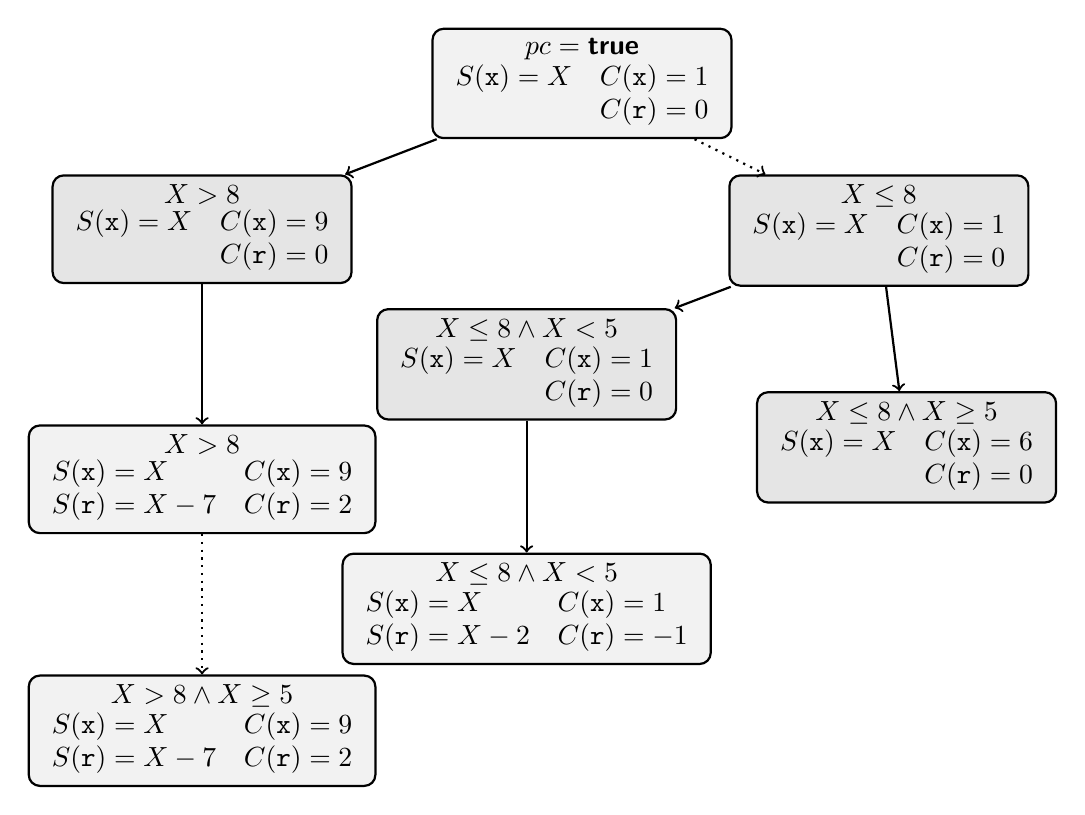
\begin{tikzpicture}[
        node distance=1.5cm and 1cm,
        every node/.style={draw, rounded corners, fill=gray!10, align=center},
        every path/.style={thick},
        decision/.style={draw, rounded corners, fill=gray!20, align=center, minimum width=3.5cm, yshift=2em}
    ]


    % Nodes
      \node (start) {\textbf{$pc = \textsf{true}$} \\
        $\begin{array}{ll}
        S(\mathtt{x}) = X & C(\mathtt{x}) = 1 \\
                          & C(\mathtt{r}) = 0
      \end{array}$ };

    \node (left)[below left=of start, decision,xshift=0em,yshift=1em] {$X > 8$ \\
        $\begin{array}{ll}
        S(\mathtt{x}) = X & C(\mathtt{x}) = 9 \\
                          & C(\mathtt{r}) = 0
      \end{array}$ };
    \node (left2)[below=of left,yshift=-0.8em] {$X > 8$ \\
        $\begin{array}{ll}
        S(\mathtt{x}) = X & C(\mathtt{x}) = 9 \\
        S(\mathtt{r}) = X-7 & C(\mathtt{r}) = 2
      \end{array}$ };
    \node (left3)[below=of left2,yshift=-0.8em] {$X > 8 \wedge X \ge 5$ \\
        $\begin{array}{ll}
        S(\mathtt{x}) = X & C(\mathtt{x}) = 9 \\
        S(\mathtt{r}) = X-7 & C(\mathtt{r}) = 2
      \end{array}$ };
      
    \node (right)[below right=of start, decision,xshift=-3em,yshift=1em] {$X \leq 8$ \\ 
        $\begin{array}{ll}
        S(\mathtt{x}) = X & C(\mathtt{x}) = 1 \\
                          & C(\mathtt{r}) = 0
      \end{array}$ };
    \node (right2)[below left=of right,decision,xshift=1em,yshift=1.5em] {$X \le 8 \wedge X < 5$ \\ 
        $\begin{array}{ll}
        S(\mathtt{x}) = X & C(\mathtt{x}) = 1 \\
                          & C(\mathtt{r}) = 0
      \end{array}$ };
    \node (right3)[below=of right2,yshift=-0.5em] {$X \le 8 \wedge X < 5$ \\ 
        $\begin{array}{ll}
        S(\mathtt{x}) = X & C(\mathtt{x}) = 1 \\
        S(\mathtt{r}) = X-2 & C(\mathtt{r}) = -1
      \end{array}$ };
    \node (right2b)[below=of right,decision,xshift=1em,yshift=-1.5em] {$X \le 8 \wedge X \ge 5$ \\ 
        $\begin{array}{ll}
        S(\mathtt{x}) = X & C(\mathtt{x}) = 6 \\
                          & C(\mathtt{r}) = 0
      \end{array}$ };
    
    % Edges
    \draw[->, dotted] (start) -- (right);
    \draw[->] (start) -- (left);
    \draw[->] (left) -- (left2);
    \draw[->,dotted] (left2) -- (left3);
    \draw[->] (right) -- (right2);
    \draw[->] (right) -- (right2b);
    \draw[->] (right2) -- (right3);
    
\end{tikzpicture}
\end{center}
Running through the program, we collect another path condition $X \ge 5$ and conjoin it
with what we had before to get $X > 8 \wedge X \ge 5$. The last possible path condition we
might explore is from negating $X \ge 5$ to yield $X > 8 \wedge X < 5$, but the SMT solver
tells us that this is unsatisfiable~(\xmark), so we are done, and we once again have the inputs
$9, 1, 6$, a.k.a. test cases \texttt{proc(9)}, \texttt{proc(1)}, and \texttt{proc(6)}.

\subsection*{A Second DART Example}
Let's now look at this code, which looks a bit more realistic. Our semantics can't quite handle it (because of the array), but we can reason through it using informal semantics.
\begin{lstlisting}
  void CoverMe(int [] a) {
    if (a == null) return;
      if (a.Length > 0)
        if (a[0] == 1234567890)
          throw new Exception("bug");
  }
\end{lstlisting}
Note again the reliance on exceptions to indicate bugs. We are trying to manufacture the non-empty
array with element 0 containing 1234567890. We start with input \texttt{null} for \texttt{a} and observe
path constraint \texttt{a == null} on that execution.

\begin{center}
\begin{tabular}{l|l|l}
  Constraints to Solve & Input & Observed constraints\\ \hline
   & \texttt{null} & \texttt{a == null}
\end{tabular}
\end{center}

We then negate the observed path constraint to get \texttt{a != null}, which we pass to the SMT solver. It creates
empty array \texttt{[]}. (It could create any array, but it's usually going to choose the simplest one first, unless you
force it not to.) At this point we have the constraint tree:

\begin{center}
  \begin{tabular}{ll}
    \begin{minipage}{.3\textwidth}
      \begin{center}
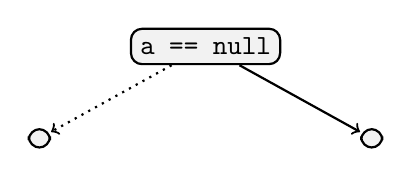
\begin{tikzpicture}[
        node distance=1.5cm and 1cm,
        every node/.style={draw, rounded corners, fill=gray!10, align=center},
        every path/.style={thick},
        decision/.style={draw, rounded corners, fill=gray!20, align=center, minimum width=3.5cm, yshift=2em}
    ]


  % Nodes
  \node (start) {\texttt{a == null}};
  \node (left) [below left=of start, text width=0.1em,yshift=2em] {};
  \node (right) [below right=of start, text width=0.1em,yshift=2em] {};

  \draw[->] (start) -- (right);
  \draw[->,dotted] (start) -- (left);
\end{tikzpicture}
      \end{center}
    \end{minipage}
&
    \begin{minipage}{.45\textwidth}
\begin{tabular}{l|l|l}
  Constraints to Solve & Input & Observed constraints\\ \hline
   & \texttt{null} & \texttt{a == null}\\ \hline
\texttt{a != null} & \texttt{[]}
\end{tabular}
    \end{minipage}
  \end{tabular}
\end{center}
We execute and monitor the function with input \texttt{a = []} and observe a new constraint
\texttt{a.Length > 0}, which evaluates to false on our input.
We once again negate the path condition to yield constraint \texttt{a != null \&\& a.Length > 0}.
We ask the SMT solver to solve that constraint and get \texttt{a = [0]}.

\begin{center}
  \begin{tabular}{ll}
    \begin{minipage}{.4\textwidth}
      \begin{center}
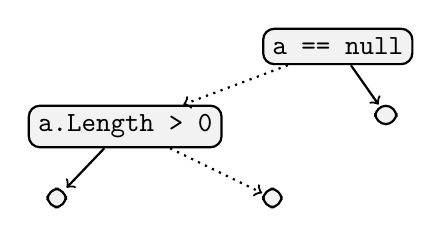
\begin{tikzpicture}[
        node distance=.5cm and .5cm,
        every node/.style={draw, rounded corners, fill=gray!10, align=center},
        every path/.style={thick},
        decision/.style={draw, rounded corners, fill=gray!20, align=center, minimum width=3.5cm, yshift=2em}
    ]


  % Nodes
  \node (start) {\texttt{a == null}};
  \node (left) [below left=of start] {\texttt{a.Length > 0}};
  \node (left1a) [below left=of left,xshift=1cm] {};
  \node (left1b) [below right=of left] {};
  \node (right) [below right=of start, text width=0.1em,xshift=-1cm] {};

  \draw[->] (start) -- (right);
  \draw[->,dotted] (start) -- (left);
  \draw[->] (left) -- (left1a);
  \draw[->,dotted] (left) -- (left1b);
\end{tikzpicture}
\end{center}
    \end{minipage}
    &
    \begin{minipage}{.45\textwidth}
\begin{tabular}{l|l|l}
  Constraints to Solve & Input & Observed constraints\\ \hline
   & \texttt{null} & \texttt{a == null}\\ \hline
  \texttt{a != null} & \texttt{[]} & \texttt{a != null}\\ 
  && ~~~ \texttt{\&\& !(a.Length>0)}\\ \hline
  \texttt{a != null \&\&} & \texttt{[0]} & \\
  ~~~ \texttt{a.Length > 0} &&
\end{tabular}
    \end{minipage}
  \end{tabular}
\end{center}
Same thing, executing and monitoring. This time we get the constraint
\texttt{a[0] != 1234567890} and add it to our constraints to solve.
That yields input \texttt{a=[1234567890]}.
\begin{center}
  \hspace*{-5em}
  \begin{tabular}{ll}
    \begin{minipage}{.4\textwidth}
      \begin{center}
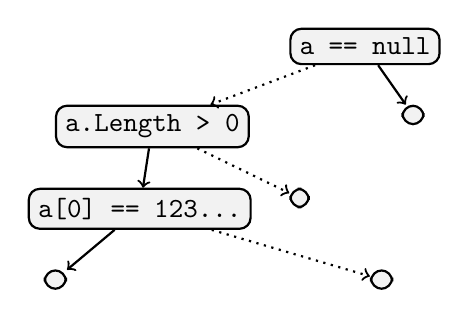
\begin{tikzpicture}[
        node distance=.5cm and .5cm,
        every node/.style={draw, rounded corners, fill=gray!10, align=center},
        every path/.style={thick},
        decision/.style={draw, rounded corners, fill=gray!20, align=center, minimum width=3.5cm, yshift=2em}
    ]


  % Nodes
  \node (start) {\texttt{a == null}};
  \node (left) [below left=of start] {\texttt{a.Length > 0}};
  \node (left1a) [below left=of left,xshift=3cm] {\texttt{a[0] == 123...}};
  \node (left1b) [below right=of left] {};
  \node (right) [below right=of start, text width=0.1em,xshift=-1cm] {};
  \node (left1aa) [below left=of left1a, text width=0.1em,xshift=1cm] {};
  \node (left1ab) [below right=of left1a, text width=0.1em,xshift=1cm] {};

  \draw[->] (start) -- (right);
  \draw[->,dotted] (start) -- (left);
  \draw[->] (left) -- (left1a);
  \draw[->,dotted] (left) -- (left1b);
  \draw[->] (left1a) -- (left1aa);
  \draw[->,dotted] (left1a) -- (left1ab);
\end{tikzpicture}
\end{center}
    \end{minipage}
    &
    \begin{minipage}{.45\textwidth}
\begin{tabular}{l|l|l}
  Constraints to Solve & Input & Observed constraints\\ \hline
   & \texttt{null} & \texttt{a == null}\\ \hline
  \texttt{a != null} & \texttt{[]} & \texttt{a != null}\\ 
  && ~~~ \texttt{\&\& !(a.Length>0)}\\ \hline
  \texttt{a != null \&\&} & \texttt{[0]} & \texttt{a != null}\\ 
  ~~~ \texttt{a.Length > 0} && ~~~ \texttt{\&\& !(a.Length>0)} \\
  && ~~~ \texttt{\&\& a[0] != 123...} \\ \hline
  \texttt{a != null \&\&} & \texttt{[123...]} &\\ 
  ~~~ \texttt{a.Length > 0} &&\\
  ~~~ \texttt{a[0]==123...} &&\\
  
\end{tabular}
    \end{minipage}
  \end{tabular}
\end{center}
We run on the final input and observe that we have achieved path coverage.
\begin{center}
  \hspace*{-5em}
  \begin{tabular}{ll}
    \begin{minipage}{.4\textwidth}
      \begin{center}
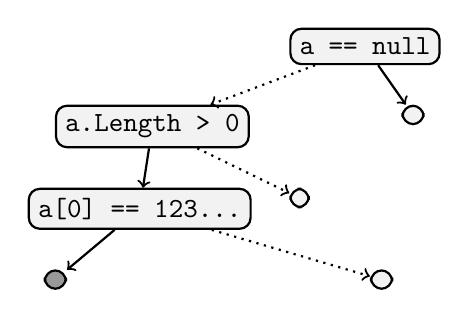
\begin{tikzpicture}[
        node distance=.5cm and .5cm,
        every node/.style={draw, rounded corners, fill=gray!10, align=center},
        every path/.style={thick},
        decision/.style={draw, rounded corners, fill=gray!20, align=center, minimum width=3.5cm, yshift=2em}
    ]


  % Nodes
  \node (start) {\texttt{a == null}};
  \node (left) [below left=of start] {\texttt{a.Length > 0}};
  \node (left1a) [below left=of left,xshift=3cm] {\texttt{a[0] == 123...}};
  \node (left1b) [below right=of left] {};
  \node (right) [below right=of start, text width=0.1em,xshift=-1cm] {};
  \node (left1aa) [below left=of left1a, text width=0.1em,xshift=1cm,fill=gray!80] {};
  \node (left1ab) [below right=of left1a, text width=0.1em,xshift=1cm] {};

  \draw[->] (start) -- (right);
  \draw[->,dotted] (start) -- (left);
  \draw[->] (left) -- (left1a);
  \draw[->,dotted] (left) -- (left1b);
  \draw[->] (left1a) -- (left1aa);
  \draw[->,dotted] (left1a) -- (left1ab);
\end{tikzpicture}
\end{center}
    \end{minipage}
    &
    \begin{minipage}{.45\textwidth}
\begin{tabular}{l|l|l}
  Constraints to Solve & Input & Observed constraints\\ \hline
   & \texttt{null} & \texttt{a == null}\\ \hline
  \texttt{a != null} & \texttt{[]} & \texttt{a != null}\\ 
  && ~~~ \texttt{\&\& !(a.Length>0)}\\ \hline
  \texttt{a != null \&\&} & \texttt{[0]} & \texttt{a != null}\\ 
  ~~~ \texttt{a.Length > 0} && ~~~ \texttt{\&\& !(a.Length>0)} \\
  && ~~~ \texttt{\&\& a[0] != 123...} \\ \hline
  \texttt{a != null \&\&} & \texttt{[123...]} & \texttt{!(a.Length>0)}\\ 
  ~~~ \texttt{a.Length > 0} &&  ~~~ \texttt{\&\& !(a.Length>0)}\\
  ~~~ \texttt{a[0]==123...} && ~~~ \texttt{\&\& a[0] == 123...}\\
  
\end{tabular}
    \end{minipage}
  \end{tabular}
\end{center}


\subsection*{SAGE: Zero to Crash in 10 Generations}
We've talked quite a bit about dynamic symbolic execution. It works in industry too. \cite{godefroid12:_sage} talks about how it's been used at
Microsoft to detect bugs in Windows, for instance to create crashing tests for a Media1 parser. (That is an easy article to read and I recommend it.) It's a lot like what we just saw. The slides do a better job
at showing this, but I'll include excerpts here.
The generation 0 seed file is all 0s:

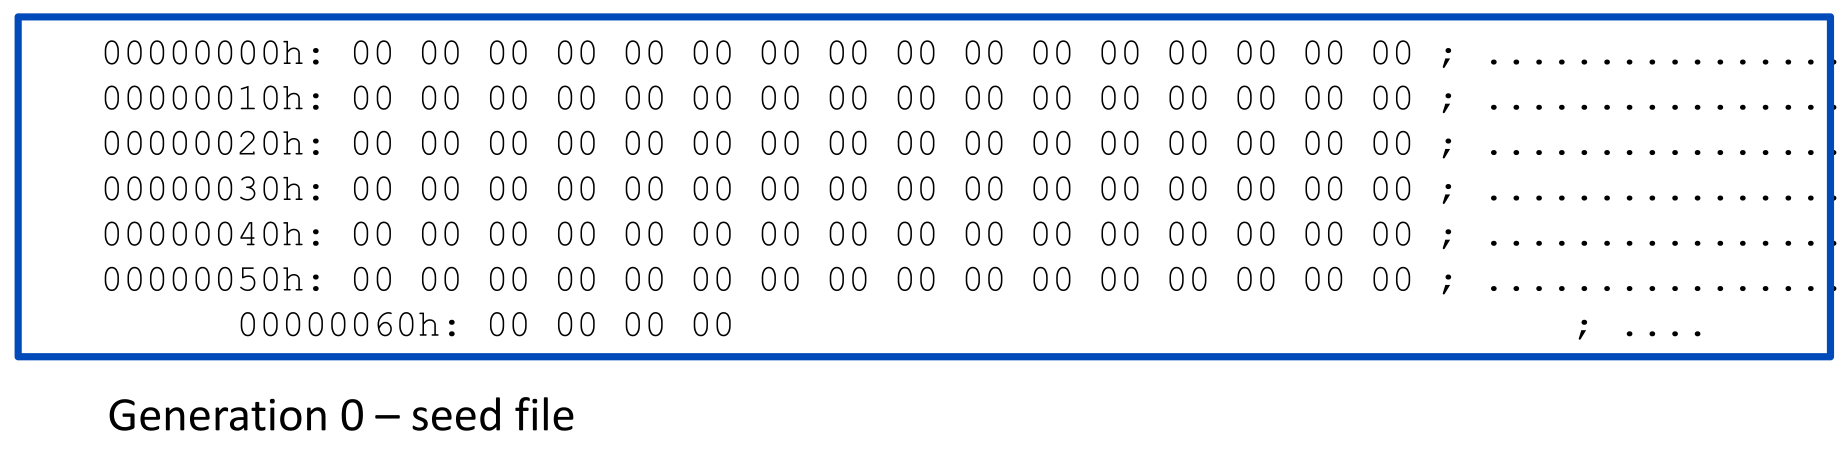
\includegraphics[width=.8\textwidth]{L09/gen0.png}

We do the same thing as we just did to get generation 1:

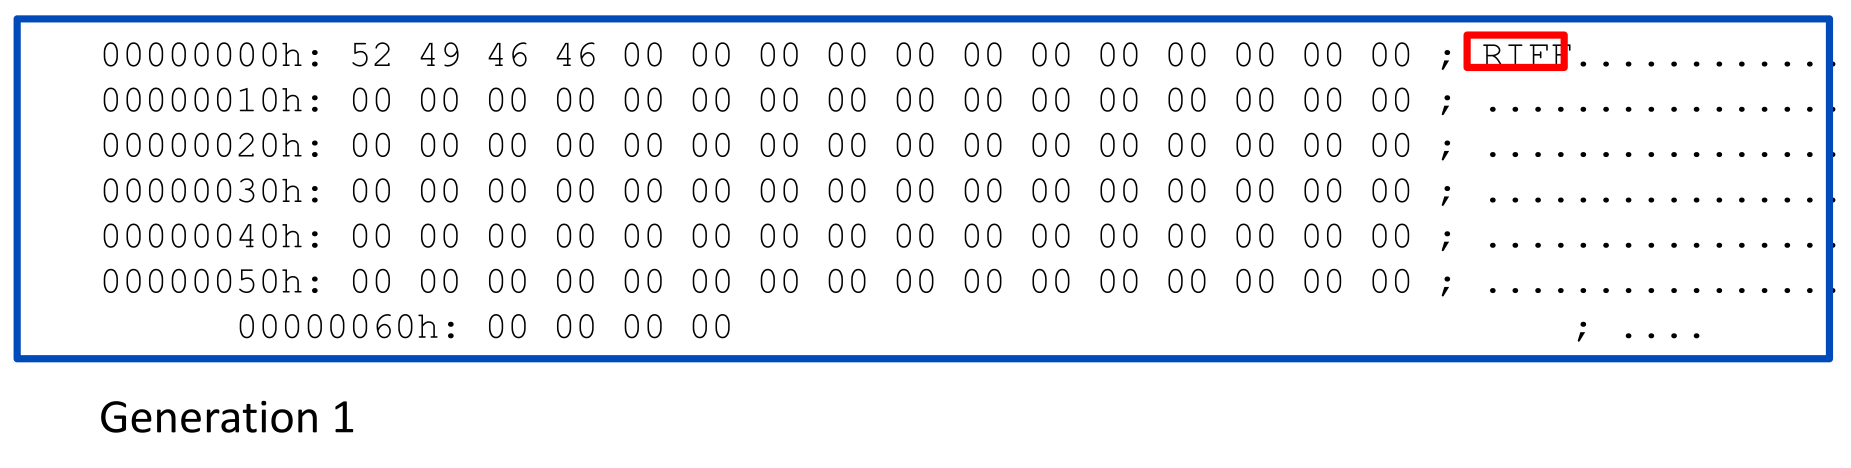
\includegraphics[width=.8\textwidth]{L09/gen1.png}

and repeat it 10 times, which yields a file that will crash the parser.

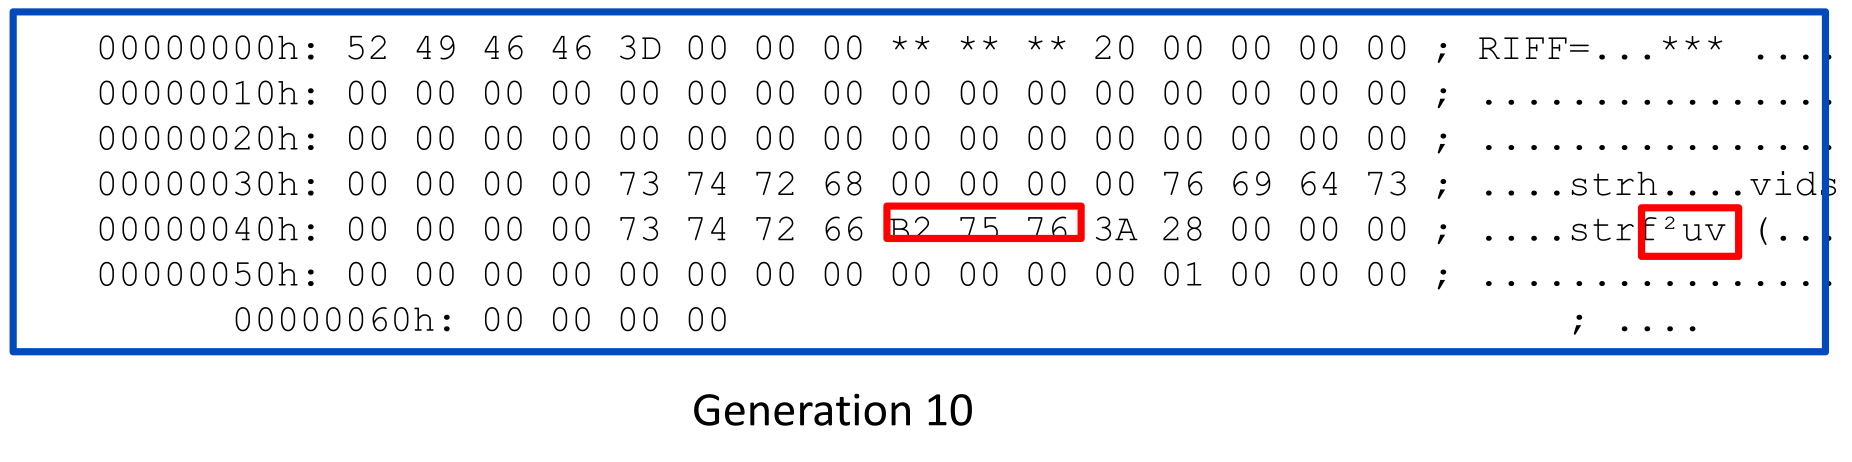
\includegraphics[width=.8\textwidth]{L09/gen10.png}

The main idea with SAGE is \emph{generational input generation}. The insight is that the thing that is expensive is the symbolic execution. SAGE uses one symbolic execution to generate multiple tests
at once. In the \texttt{CoverMe} example just above, we negated one constraint at a time, generating one new test per symbolic execution. The paper says:
\begin{quote}
  Given a path constraint,
  \emph{all} the constraints in that path are systematically negated one by one, placed in a conjunction with the prefix of the path constraint leading to it, and attempted to be solved by a constraint solver.
\end{quote}

Here's a program which we'll use to demonstate generational input generation.
\begin{lstlisting}
  void top(char input[4])
  {
    int cnt = 0;
    if (input[0] == 'b') cnt++;
    if (input[1] == 'a') cnt++;
    if (input[2] == 'd') cnt++;
    if (input[3] == '!') cnt++;
    if (cnt > 3) crash();
  }
\end{lstlisting}
We start with input \texttt{good}. This yields path constraint
\[
i[0] \neq \texttt{'b'} \wedge i[1] \neq \texttt{'a'} \wedge i[2] \neq \texttt{'d'} \wedge i[3] \neq \texttt{'!'}
\]
which then leads to four new inputs in generation 1: \texttt{bood}, \texttt{gaod}, \texttt{godd}, and \texttt{goo!}; each input is obtained from the
original input and negating a path constraint, as we've seen before, and without rerunning the symbolic execution.

We repeat the same process on all of the inputs in generation 1 to get generation 2. For this example, we can enumerate all paths
(note that this is more than branch coverage). In general there are too many paths and one quits at some point.

As for the SAGE tool itself, it was the first whitebox fuzzer used for security testing. Between 2007 and 2012 (when the paper was published), it
ran for 400+ machine years, computing over 3 billion constraints, on hundreds of apps, finding hundreds of security bugs that no other tool found.

During the development of Windows 7, SAGE found about 1/3 of all bugs discovered by file fuzzing. Even after release, it continued to find bugs,
and the fixes were quietly shipped to over 1 billion PCs.

\paragraph{DART Implementation Considerations.} Now that we've talked about generational search, we can talk about some implementation details for DART-style
dynamic symbolic execution.

Recall that the program under test is executed. That's a normal program execution, augmented with instrumentation or recording of executed instructions.
Based on the recordings, a DART-style tool will compute a path condition (or several, for generational). The ensuing symbolic execution may be computed in a separate phase (as done with SAGE)
or on-the-fly (as with CUTE/CREST).

For generational search, the path condition computation happens offline for each branch point. Since there are a lot of branch points, it's possible to create many new inputs from
a single concrete execution and symbolic execution, though the SMT solver has to be re-executed. This is easy to parallelize and distribute in the cloud.

\section{EXE versus DART}
The table you've all been waiting for.

\begin{tabular}{ll}
  \textbf{EXE} & \textbf{DART} \\
  Fine-grained control of execution & Complete execution from first step \\
  Shallow exploration  & Deep exploration  \\
  ~~~ (many queries early on) & ~~~ (one query per run) \\
  Online symbolic execution  & Offline SE possible \\
  ~~~ (SE and interpretation in lockstep) & ~~~  (execute along recorded trace)
\end{tabular}

\section{Loops: Dynamic Symbolic Execution Doesn't Solve All Problems}
Loops are a problem for symbolic execution. Symbolic execution can only reason about finitely many execution steps.
Programs have loops and may execute for arbitrarily many steps.
(Recall that when we write proofs about loops, we need invariants).

One way to handle this is to dynamically unroll loops. That is,
copy-paste the loop body $N$ times in a row, for some finite $N$.  One
would treat the backwards conditional branch implementing the loop as
a branch condition for symbolic execution, and the choices are to do
one more loop iteration, or to exit the loop.

If a loop can only run some small (finite) number of iterations, then
unrolling can completely explore the behaviour of that loop.  (This is
also a key idea behind bounded model checking, which we'll discuss
later).

Other loops can run unbounded numbers of iterations (e.g. just about
any operation on a collection data structure). Symbolic execution will
either get stuck or skip such loops. More powerful techniques are
needed.

Actually, only loops whose iteration count depends on the input are
problematic. If we know the maximum iteration count, then it's
possible to execute the loop concretely.

\paragraph{Dynamic Symbolic Execution and Input-Dependent Loops.} Here's some options to handle loops.

In EXE (online symbolic execution), then every iteration of the loop forks the execution, and the search algorithm (at runtime) can get bored and
break out, or it can continue unrolling the loop and running one more iteration.

In DART (offline symbolic execution), we have an input and hence a concrete trace. The trace encodes some number of unrollings. Then, the search algorithm
can cause a different number of loop executions by flipping one of the loop branches.

In either case, a na\"ive search algorithm might get stuck.

\section{Concretization}
Continuing on the ``dynamic symbolic execution doesn't solve all problems'' theme, let's think about this. DSE executes the program both concretely and symbolically.
\begin{itemize}[noitemsep]
\item concrete execution is ``easy'' (just get a VM to do it)
\item symbolic execution can be hard (e.g. multiplication)
\end{itemize}
What can we do when symbolic reasoning is too hard? One answer is \emph{concretization}.

In concretization, we selectively replace symbolic inputs by concrete values.
\begin{itemize}[noitemsep]
\item this simplifies symbolic reasoning; concrete expressions are easy, we said, and we can make a symbolic expression easier to reason about by substituting in concrete values. At the limit, if we replace all symbolic variables, then the operational semantics gives a concrete value for any expression.
\item but, how do we know what to concretize? It's not always clear why an expression is hard to symbolically reason about.
\item concretization can result in \emph{unsoundness}; to mitigate this, we must record the concretization decision in the path condition;
\item concretization will definitely result in \emph{incompleteness}: we had all possible values of $X$ and now we just have 5. What about $X = 6$? Or $X=-5$?
\end{itemize}

\paragraph{Example.} Let's do a concretization. Here's a state and a program.

\begin{tabular}{ll}
  \begin{minipage}{.5\textwidth}
    \begin{tabular}{ll}
      \multicolumn{2}{c}{$\textit{true}$} \\ \hline
      & $C(X) = 5$ \\
      $S(\texttt{m}) = X + 2$ & $C(\texttt{m}) = 7$ \\
      $S(\texttt{size}) = Y$ & $C(\texttt{size}) = 256$
    \end{tabular}
  \end{minipage}
  &
  \begin{minipage}{.4\textwidth}
  \begin{lstlisting}[numbers=none]
    if (m*m > size) {
      // ...
  \end{lstlisting}
  \end{minipage}
\end{tabular}

The program contains condition \texttt{m*m > size}, which expands to
symbolic $(X+2)(X+2) > Y$.

It turns out that symbolic multiplication
is difficult for SMT solvers. We therefore choose to concretize
variable $X$, using its current concrete value $C(X) = 5$.
The condition therefore becomes $49 = (5+2)(5+2) > Y$.

If we want to enter the then-branch of the if statement,
we do as usual: update the path condition with the (concretized)
branch condition $49 > Y$, solve for symbolic input $Y$, and get
e.g. $Y = 48$.

\begin{tabular}{ll}
  \begin{minipage}{.5\textwidth}
    \begin{tabular}{ll}
      \multicolumn{2}{c}{$49 > Y$} \\ \hline
      & $C(X) = 5$ \\
      $S(\texttt{m}) = X + 2$ & $C(\texttt{m}) = 7$ \\
      $S(\texttt{size}) = Y$ & $C(\texttt{size}) = 48$
    \end{tabular}
  \end{minipage}
  &
  \begin{minipage}{.4\textwidth}
  \begin{lstlisting}
    if (m*m > size) {
      // ...
  \end{lstlisting}
  \end{minipage}
\end{tabular}

Now say that inside the then-branch we furthermore have \texttt{if (m < 5)}.
Symbolically, this works out to $X + 2 < 5$ due to the symbolic value for \texttt{m}.
To explore this then-branch, we'd ask the SMT solver for a solution, and we could well get
$X = 2$. But that's wrong. We had concretized $X$ to 5, and now we're saying that $X$ has to be 2.

\textbf{How to avoid this:} record $X = 5$ in the path condition when you concretize. The SMT solver might then say ``no solutions'' (you're missing behaviours that you concretized away), but you won't get wrong results.

\paragraph{Concretization Algorithm.}
Here's an algorithm for concretizing variables in a symbolic expression, which you might use when the expression is too hard to deal with.
As input:
\begin{itemize}[noitemsep]
\item a state, including path condition $\mathit{pc}$ and concrete and symbolic states $C$ and $S$;
\item a symbolic expression $E$ to concretize
\end{itemize}
The algorithm:
\begin{itemize}[noitemsep]
\item choose variables $x_1, \ldots, x_k$ in $E$ to concretize;
\item let $E'$ be the result of replacing $x_i$ by $C(x_i)$ in $E$;
\item add the concretization constraint $x_1 = C(x_1) \wedge \cdots \wedge x_k = C(x_k)$ to $\mathit{pc}$;
\item return the result of evaluating $E'$ on symbolic state $S$.
\end{itemize}

\paragraph{Soundness and Completeness.} Conceptually, each path that you explore in the dynamic symbolic execution is exact. The concrete results are concrete, and the
symbolic state is computing what is called the strongest postcondition. There's no approximation here, on a per-path basis.

But, symbolic execution (static or dynamic) doesn't guarantee that you explore all of the paths (remember what we said about loops); it underapproximates. In finite time, you only visit a subset
of the paths. There is a sort of ``eventual'' completeness in that if you let it run for long enough, you'll observe any behaviour that is possible. It's sound, in that you don't see anything
that is infeasible.

Concretization remains sound (if you modify the path condition as stated above). But you are exploring less. In particular, you lose the eventual completeness property mentioned above.

\paragraph{Summary of concretization.}
This technique, concretization, is a key technique for making dynamic symbolic execution work in practice. It enables external calls, which you can't evaluate symbolically. You can evaluate
the calls if you concretize the call arguments and just call the callee.

We talked about concretization constraints. It is possible to not add them to the path condition, as was done in the original DART. Then the dynamic symbolic execution might diverge
when it has contradictory values for symbolic variables. This isn't sound. But if you are willing to sacrifice soundness, you can deal with divergences with random restarts.

\bibliographystyle{alpha}
\bibliography{L09}

\end{document}
